%% content.tex
%%

%% ===========================
\chapter{Grundlagen}
\label{ch:grundlagen}
%% ===========================

%% ===========================
\section{NoSQL - Eine Einführung}
\label{ch:grundlagen:sec:NoSQL}
%% ===========================

NoSQL ist keine Datenbank, noch nicht einmal ein Datenbanktyp. Der Terminus NoSQL fasst lediglich Datenbank zusammen die nicht dem Model der relationalen Algebra folgen. Eines haben Sie jedoch Gemeinsam, die treibende Idee die zu Ihrer Entwicklung geführt hat. Die Entstehung der NoSQL Datenbanken ist auf die schlechte Horizontale Skalierbarkeit von relationalen Datenbanken zurückzuführen. Verfügbarkeit und Skalierbarkeit sind unter gewissen Umständen wichtiger als Atomarität und Konsistenz. NoSQL Datenbanken lassen sich anhand Ihres Datenmodells unterscheiden. Nach \cite{vaish2013getting} ist eine Klassifizierung in folgenden Kategorien möglich:

%% ===========================
\subsection{Document Stores}
\label{ch:grundlagen:sec:NoSQL:DocumentStores}
%% ===========================

Document Stores koppeln komplexe Datenstrukturen (Dokumente) mit einem eindeutigen Schlüssel. Der Datenzugriff findet dabei in der Regel über das HTTP-Protokoll mit REST-API oder über das Apache Thrift-Protokoll statt \cite{agarwal2007thrift}. In Documents Stores gibt es außerdem kein Schema. Statt jeden Datensatz in einer Zeile bestehend aus Spalten zu speichern, wird Sie in einem Dokument abgelegt. Diese können als eine Datei auf dem Dateisystem betrachtet werden. Dieses Dokument kann alle möglichen Daten aufnehmen und muss dabei keinem Schema folgen. Obwohl die Daten schemalos sind, sind sie sind nicht frei von formellen Restriktionen. Die meisten der verfügbaren Datenbanken unter dieser Kategorie benutzen XML, JSON, BSON oder YAML. Document Stores eignen sich wenn dynamische Entitäten eingesetzt werden die z.B. eine hohe Anzahl von optionalen Feldern besitzen.

%% ===========================
\subsection{Extensible Record Store}
\label{ch:grundlagen:sec:NoSQL:ExtensibleRecordStore}
%% ===========================

Extensible Record Stores, auch Wide Column Stores und auf deutsch oft spaltenorientierte Datenbank genannt, speichern im Gegensatz zu den traditionellen relationalen Datenbanken, Daten mehrerer Einträge in Spalten anstatt in Zeilen. Jeder Eintrag einer Spalte besteht aus einem Namen, den Daten und einen Zeitstempel.

In Extensible Record Stores werden sogenannte Spalten Familien zur Gruppierung ähnlicher oder verwandter Inhalte verwendet. In Abbildung \ref{wide_column_store} ist eine solche Spalten-Familie zu sehen. Spalten Familien besitzen keine logische Struktur und geben somit kein Schema vor. Weiterhin können die Struktur tausenden oder sogar Millionen von Spalten beinhalten weshalb sie auch Wide Columns Stores genannt werden. Verwandten Spalten werden in Spalten-Familien durch von einer Anwendung bereitgestellte Reihe von Schlüsseln identifiziert. Weiterhin muss in einer Spalten-Familie nicht jede Zeile aus den gleichen Spalten bestehen.

\begin{figure}[H]
	\centering
  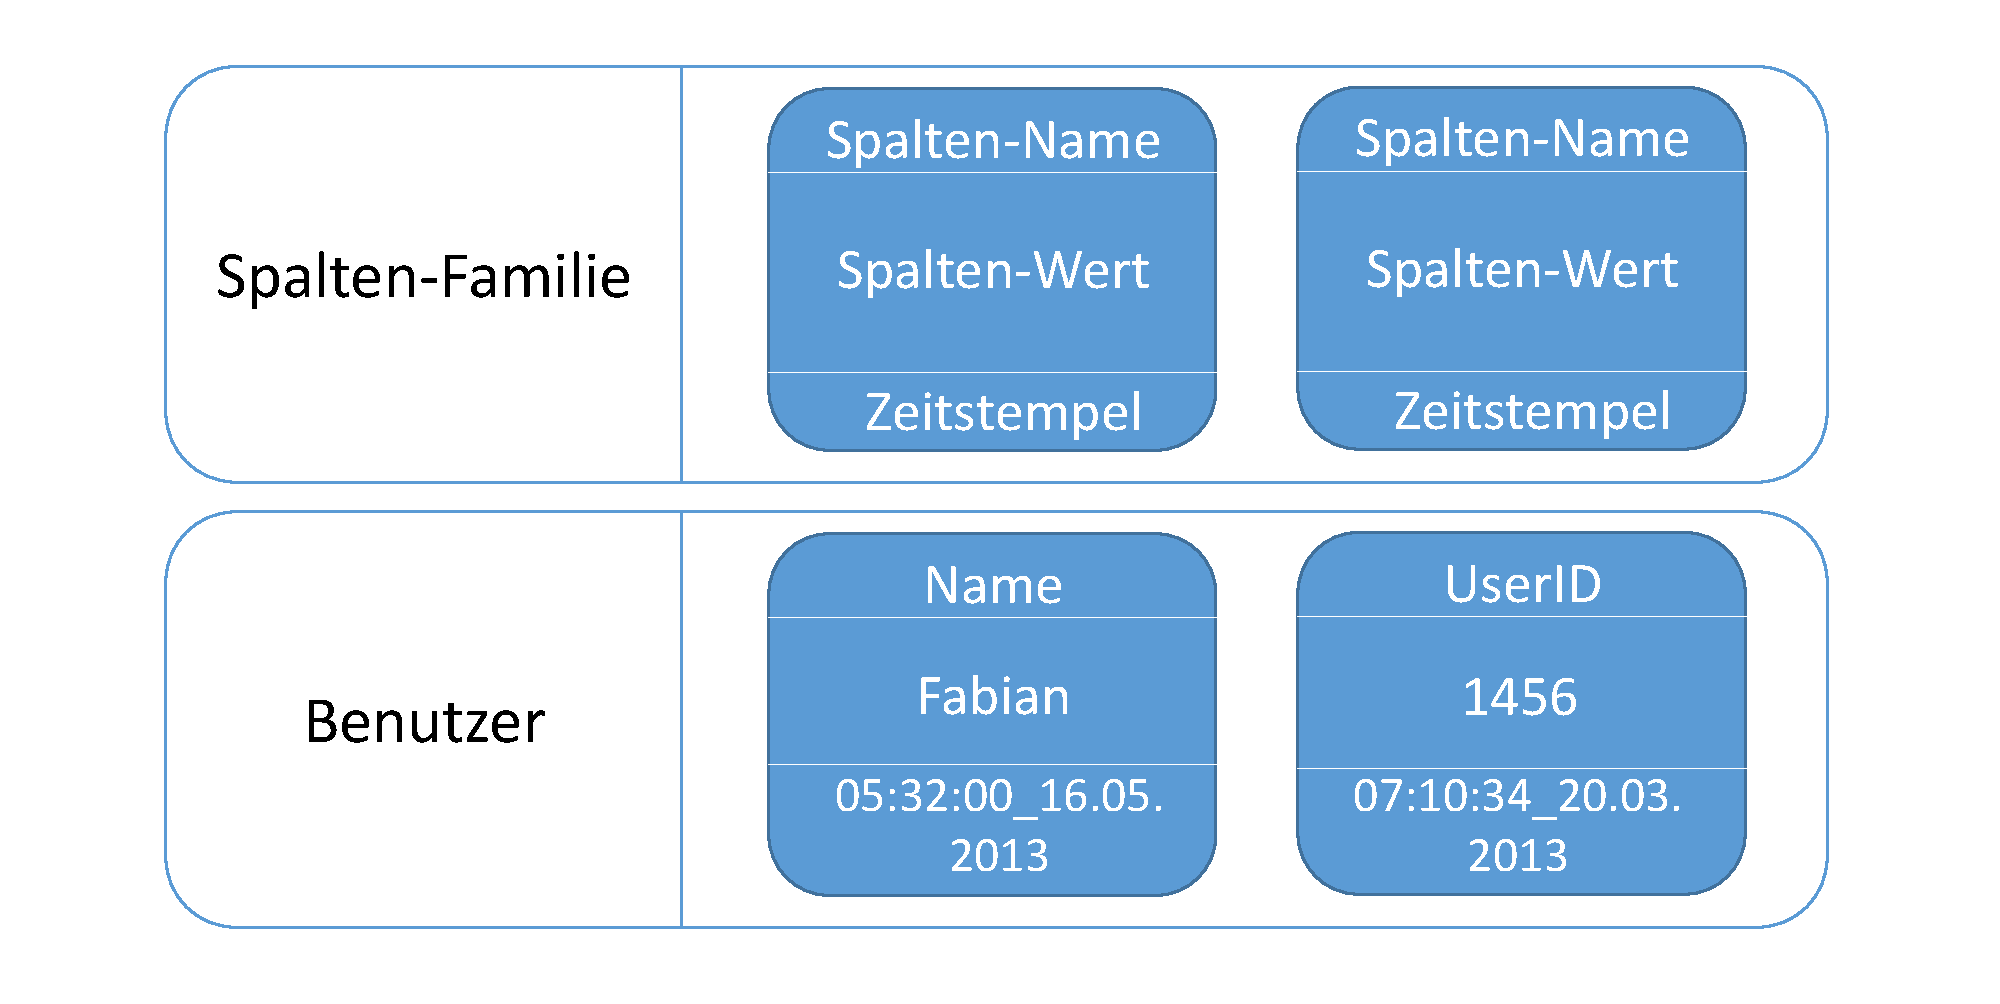
\includegraphics[width=0.8\textwidth, width=0.8\textwidth]{pics/wide_column_stores.pdf}
	\caption{Beispiel einer Spalten Familie}
	\label{wide_column_store}
\end{figure}

Diese Architektur hat mehrere Vorteile. Meist weisen Werte in Spalten eine geringe Entropie auf was Sie geeignet für Kompressionsverfahren macht. Die Verarbeitung der Anfragen wird ebenfalls beschleunigt da keine unnötigen Informationen gelesen werden. Dies trifft in der Regel für Lese- und Schreibprozesse zu, wenn es um eine einzelne Spalte geht (in der Regel ein disk-seek). Performance verschlechternd sind natürlich im Gegenzug Zugriffe die nicht mehr auf einzelnen Spalten erfolgen sondern über viele Spalten hinweg ausgeführt werden.

%% ===========================
\subsection{Key-Value-Store}
\label{ch:grundlagen:sec:NoSQL:KeyValueStore}
%% ===========================

Key-Value-Stores sind die einfachsten NoSQL-Datenbanken. Sie ermöglichen die Speicherung von Werten mit einem Schlüssel. Im Gegensatz zu relationalen Datenbanken, haben Key-Value-Stores keine Kenntnis von den Daten in den Werten und sind daher schemafrei. Grundsätzlich trifft das auf die meisten Umsetzungen von Key-Value-Stores zu. Redis und andere Umsetzungen sind allerdings in der Lage strukturiere Daten abzulegen und Ihre Felder zu indexieren. Dadurch wird die Komplexität solcher Datenbank gesteigert was jedoch nicht dazu führt das sie Join- oder Aggregat-Operatoren beherrschen. 

%% ===========================
\subsection{Graph Datenbanken}
\label{ch:grundlagen:sec:NoSQL:GraphDatenbanken}
%% ===========================

Eine Graph Datenbank verwendet die Graphen Theorie zur Abbildung und Abfrage von Beziehungen \cite{SWB-386976589}. Im Grunde besteht eine solche Datenbank aus einer Menge von Knoten und Kanten. Jeder Knoten repräsentiert dabei eine Entität und jede Kante eine Beziehung oder Verbindung zwischen zwei Knoten, wie in Abbildung \ref{graph_database} zu sehen. Knoten definieren sich durch einen sogenannten unique identiefier, sowie durch die Anzahl abgehenden und/oder eingehenden Kanten  und einer Menge von Attributen. Kanten werden wie Knoten definiert nur das sie Anstatt Kanten, einen Start- und End-Knoten besitzen. Graph-Datenbanken eignen sich gut für die Analyse von Verbindungen, weshalb sie oft zur Datengewinnung im Social Media Umfeld genutzt werden.

\begin{figure}[H]
	\centering
  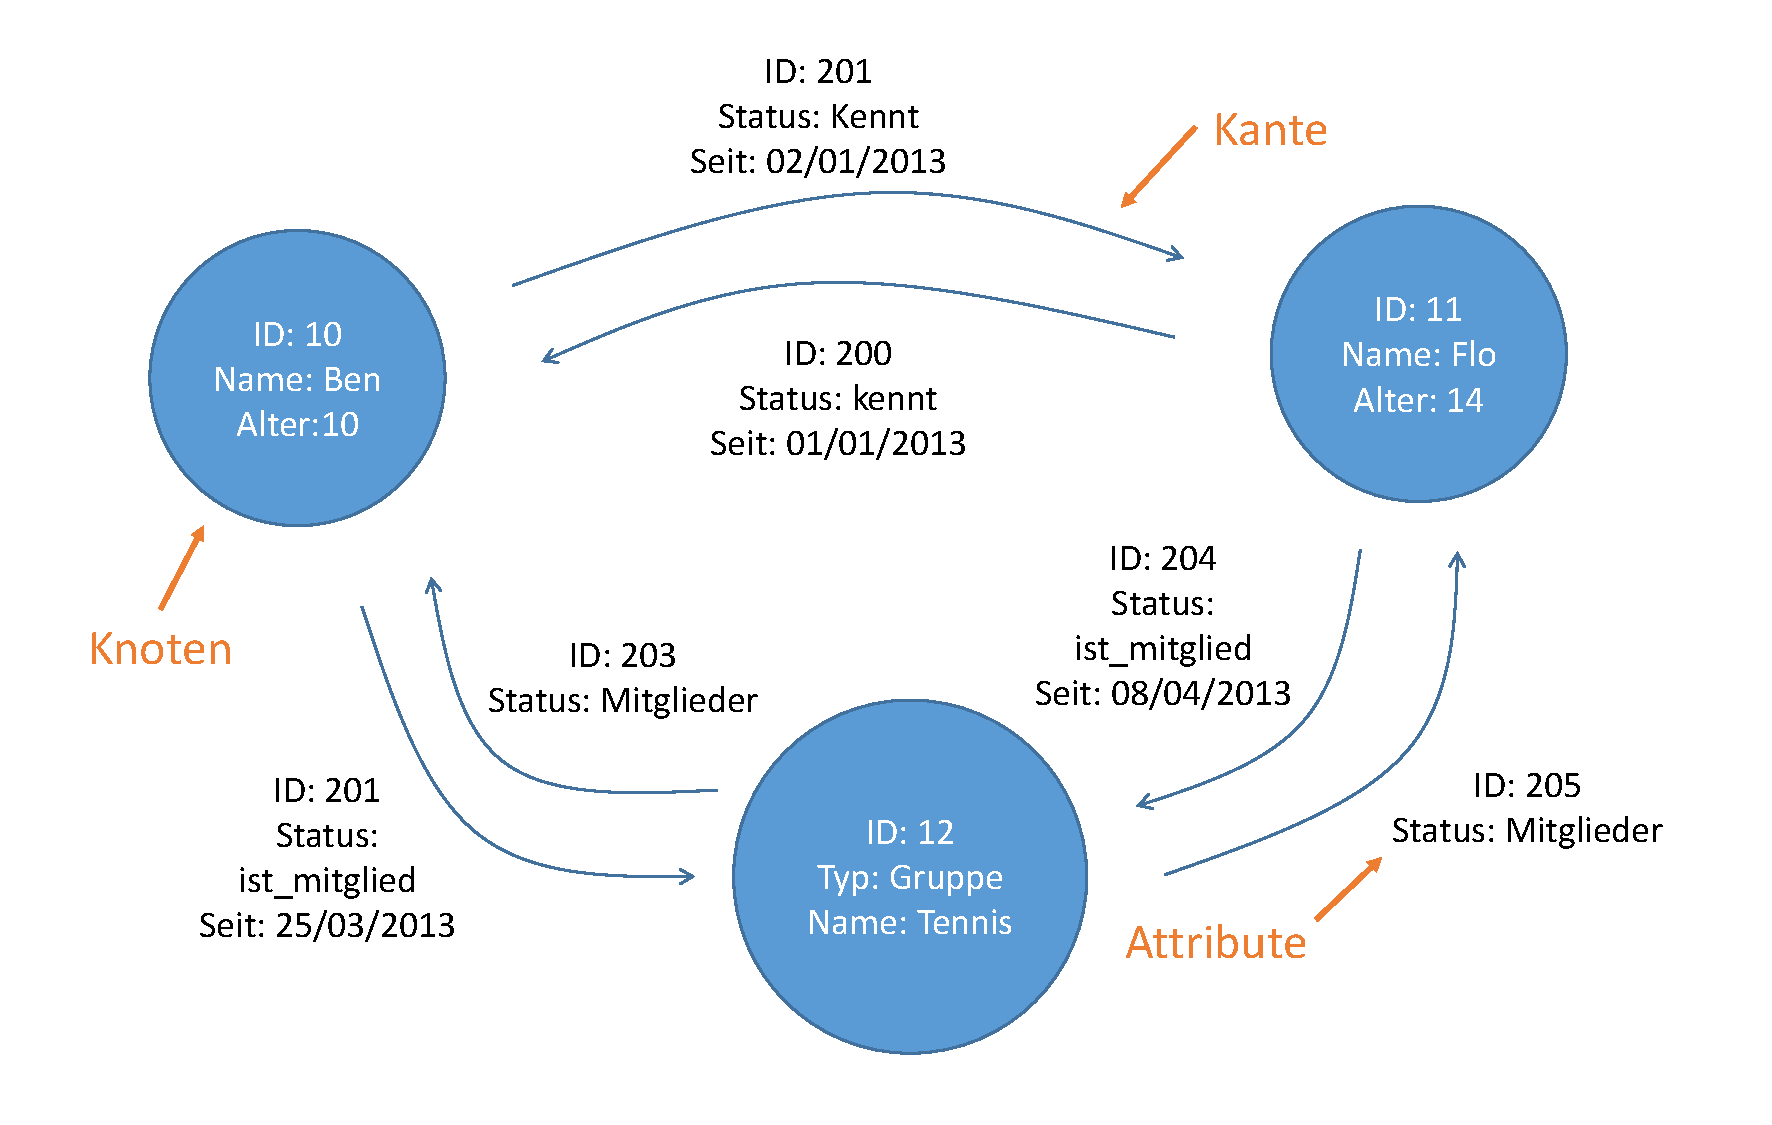
\includegraphics[width=1.0\textwidth, width=1.0\textwidth]{pics/graphdatabase.pdf}
	\caption{Beispiele von Knoten und Kanten in einer Graph Datenbank}
	\label{graph_database}
\end{figure}

%% ===========================
\subsection{NoSQL Theoretische Grundlagen}
\label{ch:grundlagen:sec:NoSQL:NoSQLBasics}
%% ===========================

Im nachfolgenden werden Begriffe und Verfahren erläutert die durch die NoSQL Bewegung geprägt wurden.

\paragraph{Replikation} Replikation im Falle von verteilten Datenbanken bedeutet, dass ein Datenelement an mehr als einem Knoten gespeichert ist. Dies ist sehr nützlich, um Lese-Performance der Datenbank zu erhöhen, weil es einen Load Balancer erlaubt alle Lesevorgänge über viele Maschinen zu verteilen. Außerdem ist von Vorteil, dass es die Cluster robuster gegen den Ausfall einzelner Knoten macht.

\paragraph{Fragmentierung} Fragmentierung in der Datenbank ist der Zustand bei dem die Daten in mehrere Fragmente aufgeteilt wurden. Diese können dann über viele Knoten verteilt werden. Die Datenpartitionierung kann beispielsweise mit einer konsistenten Hash-Funktion erfolgen, die auf dem Primärschlüssel der Datenelemente angewendet wird um das zugehörige Fragment zu bestimmen.

\paragraph{Eventuelle Konsistenz} Später in diesem Kapitel wird das CAP-Theorem eingeführt, was die Implikation hat
dass die verteilten Datenbanken entweder stark konsistent oder verfügbar sein können. Folglich können die meisten NoSQL Datenbanken nur eventuelle Konsistenz bieten, eine abgeschwächte Art der starken Konsistenz. Starke Konsistenz bedeutet, dass alle mit der Datenbank verbundenen Prozesse immer die gleiche Version sehen. Eventuelle Konsistenz ist schwächer und garantiert nicht, dass jeder Prozess die selbe Version sieht.

\paragraph{Multiversion Concurrency Control (MVCC)} MVCC ist eine effiziente Methode mehrere Prozesse auf dieselben Daten parallel zugreifen zu lassen ohne eine Beschädigung der Daten und die Möglichkeit von Deadlocks. Es ist eine Alternative zu den Lock-basierte Ansätzen, wobei jeder Prozess zuerst eine exklusive Sperre auf einem Datenelement anfordern muss, bevor es gelesen oder aktualisiert werden kann. Zu diesem Zweck werden intern verschiedene Versionen eines Objektes gehalten.

\paragraph{MapReduce} MapReduce ist ein von Google entwickeltes Programmiermodell für verteilte Berechnungen und ist in einem Papier von Dean und Ghemawat \cite{Dean:2008:MSD:1327452.1327492} beschrieben. Anwendungen, die mit dem MapReduce-Framework geschrieben werden, können automatisch auf mehreren Computern verteilt werden ohne dass der Entwickler benutzerdefinierte Code für die Synchronisation und Parallelisierung schreiben muss. Es kann verwendet werden um Aufgaben auf großen Datenmengen durchzuführen, die zu groß für eine einzelne Maschine zu handhaben wären.


\paragraph{Vector Clocks (Vektor Uhren)}
Vektor Uhren basieren auf der Arbeit von Lamport \cite{Lamport:1978:TCO:359545.359563} und werden von vielen Datenbanken verwendet, um festzustellen ob ein Datenelement durch konkurrierende Prozesse verändert wurde. Jedes Datenelement besitzt eine Vektor Uhr welche aus Tupeln mit verschiedenen Zeitpunkten besteht. Jeder Zeitpunkt stellt einen Prozess der eine Modifikation an dem Datenelement vorgenommen hat dar. Jede Uhr beginnt bei Null und wird durch seinen Prozess bei jedem Schreibvorgang erhöht. Um den eigenen Wert der Uhr zu erhöhen, verwendet der Schreibprozess das Maximum aller Uhrenwerte im Vektor und erhöht sie um eins. Wenn zwei Versionen eines Elements zusammengeführt werden, können die Vektoruhren benutzt werden um Konflikte zu erkennen. Wenn mehr als eine Uhr differenziert muss ein Konflikt vorhanden sein. Wenn es keinen Konflikt gibt, kann die aktuelle Version durch den Vergleich der Maxima der Uhren ermittelt werden.

\paragraph{Das CAP Theorem} Das CAP-Theorem wurde von Dr. Brewer erstmal in einem Symposium \cite{cap2010} über den Trade-Off in verteilten Systemen eingeführt und wurde später von Gilbert und Lynch \cite{Gilbert:2002:BCF:564585.564601} formalisiert. Es besagt, dass in einem verteilten Datenspeichersystem nur zwei Merkmale aus Verfügbarkeit, Konsistenz und  Partitionstoleranz garantiert werden können. Verfügbarkeit bedeutet in diesem Fall, dass die Clients in einem bestimmten Zeitraum immer Daten lesen und schreiben können. Eine Partition tolerante verteilte Datenbank ist fehlertolerant gegen temporäre Verbindungsprobleme und ermöglicht es Partitionen über Knoten zu trennen. Ein System das tolerant partitioniert ist kann nur starke Konsistenz durch Verminderungen in seiner Verfügbarkeit erreichen. Grund dafür ist das es zuerst sicherstellen muss ob jeder Schreibvorgang abgeschlossen wurde bevor er eine Replikation durchführen kann. Jedoch kann es vorkommen das in einer verteilten Umgebung das nicht möglich ist, Aufgrund von Verbindungsfehlern oder anderen temporären Hardware Problemen.

%% ===========================
\section{In Memory Datenbanken}
\label{ch:grundlagen:sec:InMemoryDatenbanken}
%% ===========================

Eine In-Memory-Datenbank (IMDB) ist ein Datenbank-Management-System, das in erster Linie den Hauptspeicher als Medium für die Datenablage benutzt. Eine IMDB wird auch als Hauptspeicher-Datenbank (MMDB) oder Echtzeit -Datenbank (RTDB) bezeichnet. IMDBs sind schneller als die Festplatten optimierte Datenbanken, denn sie führen weniger CPU-Befehle aus und ihre internen Optimierungsalgorithmen sind viel einfacher gestaltet. Einsatz finden Sie vor allem in Anwendungen, bei denen Reaktionszeit von entscheidender Bedeutung ist. Mehrkernprozessoren, 64-bit Architekturen und gesunkene RAM Preise stellen die treibenden Faktoren in der Entwicklung solcher Systeme dar \cite{SWB-381840476}.

Die hohe Performance dieser Systeme kann nicht durch simples verschieben der Daten in den Hauptspeicher erreicht werden. Bisherige Konzepte des Datenbankentwurfs müssen dabei neu überdacht werden. In herkömmlichen Datenbanken ist der Speicherverbrauch kein relevanter Faktor. In IMDBs hingegen ist der Einsatz von Speicherplatz sparenden Maßnahmen eine Notwendigkeit. Dictionary Encoding, Run-Length Encoding oder Cluster Encoding sind nur einige Techniken zur Reduktion des Speicherplatzverbrauches. Solche Techniken bieten sich vor allem in spaltenorientierten Systemen aufgrund der geringen Entropie innerhalb der Spalten an \cite{Abadi:2006:ICE:1142473.1142548}. Neben den Optimierungsansätzen in der Datenhaltung können Regeln formuliert werden um nicht mehr verwendete Daten zu erkennen. Dabei kann z.B. zwischen aktiven Daten (Daten von nicht abgeschlossenen Geschäftsprozessen) und passiven Daten (Daten von abgeschlossenen Geschäftsprozessen) unterschieden werden. Wenn ein Geschäftsprozess in sich abgeschlossen ist werden die Daten nur noch aus Datenvorhaltungsgründen aufbewahrt. Eine Auslagerung solcher nicht benötigten Daten ermöglicht es zusätzlichen Speicherplatz Verbrauch zu reduzieren.
 
In-Memory Datenbanken die den relationalen Ansatz verfolgen besitzen zudem geänderte Query Optimierer. In herkömmlichen RDBMS sind Lese- und Schreiboperationen einer der wichtigsten Faktoren zur Bestimmung des optimalen Query Plans. Sie spielen jedoch eine stark untergeordnete Rolle in IMDB. Im Gegenzug nimmt die Reduktion von CPU-Zyklen einen höheren Stellenwert ein.

In traditionellen Datenbanken stellt das Wiederherstellen aufgrund des nicht flüchtigen Speichers kein Problem dar. IMDB müssen dagegen für den Fall eines Systemausfalls Snapshot Dateien anlegen. Diese werden zur Wiederherstellung des Datenbestandes benötigt. Snapshot sind Abbilder des aktuellen Datenbestandes. Um Rücksicht auf die Performance zu nehmen werden die Snapshots entweder in Intervallen oder zu festgelegten Ereignissen erzeugt. Damit Veränderungen an Daten zwischen Snapshots nicht verloren gehen, werden Sie in Logg Dateien zwischengespeichert. Zusammen mit den Snapshots dienen sie als Grundlage für die Datenwiederherstellung. 

%% ===========================
\section{Component Object Model}
\label{ch:grundlagen:sec:ComponentObjectModel}
%% ===========================

Component Object Model (COM) ist ein binärer-Schnittstellenstandard für Software-Komponenten der von Microsoft im Jahr 1993 eingeführt wurde \cite{SWB-088582566}. Er wird verwendet, um Interprozesskommunikation und dynamische Objekterstellung in einer Vielzahl von Programmiersprachen zu ermöglichen. Um zu verstehen was COM ist (und damit alle COM-basierten Technologien), ist es wichtig zu verstehen, dass es sich nicht um eine objektorientierte Sprache, sondern um einen Standard handelt. Er definiert nicht die Sprache, Struktur oder Implementierungsdetails. Jeder dieser Entscheidungen werden dem Programmierer überlassen. Es spezifiziert lediglich ein Objekt Model und die Anforderungen an die Kommunikationen zwischen COM-Objekten und anderen Objekten. Es spielt dabei keine Rolle ob Objekte sich im gleichen oder in unterschiedlichen Prozessen befinden. Sie können sogar auf unterschiedlichen Rechner laufen. Die Umsetzung in verschiedenen Sprachen ist durch die Umsetzung der Kommunikation in binären Maschinen Code möglich. Das führt dazu das COM des Öfteren als binärer Standard referenziert wird.

COM bietet die Möglichkeit auf viele Windows Funktionen zuzugreifen. Des weiteren ist COM die Basis für die OLE–Automation (Object Linking and Embedding) und ActiveX. Die Verwendung des COM-Standards bietet weiterhin folgende Vorteile:

\begin{itemize}
\item Sprachunabhängig
\item Versionsunabhängig
\item Plattformunabhängig
\item Objektorientiert
\item Ortsunabhängig
\item Automatisiert
\end{itemize} 

%% ===========================
\subsection{Architektur}
\label{ch:grundlagen:sec:ComponentObjectModel:subsec:Architektur}
%% ===========================

COM basiert auf dem Client/Server-Prinzip. Wie in Abbildung \ref{GL_COM} zu sehen erzeugt ein COM-Client, eine COM-Komponente in einem so genannten COM-Server und nutzt die Funktionalität des Objektes über COM-Schnittstellen. 

\begin{figure}[H]
	\centering
  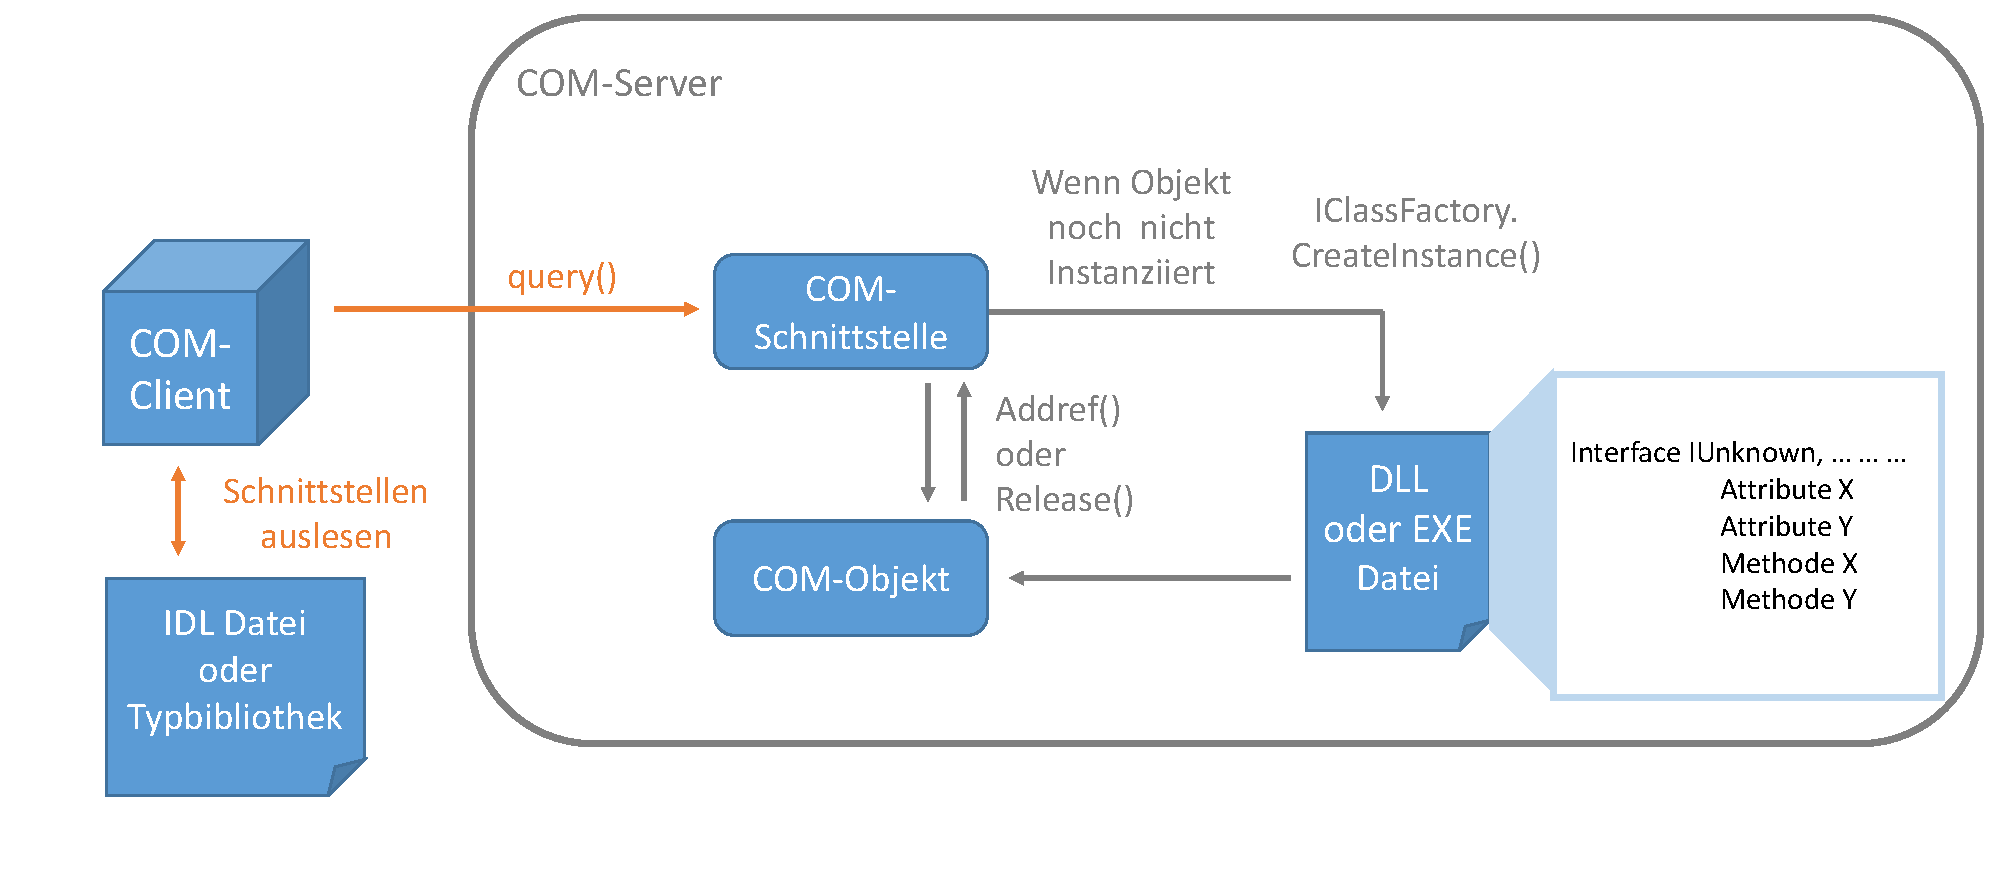
\includegraphics[width=1.0\textwidth, width=1.0\textwidth]{pics/Grundlagen_com.pdf}
	\caption{Bestandteile einer COM-Architektur}
	\label{GL_COM}
\end{figure} 

%% ===========================
\subsection{COM-Client}
\label{ch:grundlagen:sec:ComponentObjectModel:subsec:COMClient}
%% ===========================

Der COM-Client stellt den Benutzer einer COM-Komponente dar. Die Nutzung der COM-Komponenten erfolgt über sogenannte Interfaces. Interfaces werden über Typbibliotheken veröffentlicht oder stehen in Form von Beschreibungen in der IDL (Interface Definition Language) zu Verfügung. Clients steht außerdem die Möglichkeit einer Query zur Verfügung, mithilfe er feststellen kann ob ein Objekt das angefragte Interface unterstützt. Dabei wird lediglich die Query-Operation mit einer GUID als Parameter auf dem ausgewähltem Objekt ausgeführt. Falls das Objekt das geforderte Interface unterstützt liefert es den entsprechenden Pointer zum Interface zurück.  

%% ===========================
\subsection{COM-Server}
\label{ch:grundlagen:sec:ComponentObjectModel:subsec:COMServer}
%% ===========================

Ein COM-Server wird durch eine DLL oder ausführbare Datei realisiert, die eine COM-Komponente beinhaltet oder bereitstellt. Dabei unterscheidet man zwischen 3 Arten von COM-Servern. Die erste Variante ist der In-process-Server der sich dadurch auszeichnet das er beim Instanzieren einer COM-Komponente mit in den Prozess der Anwendung (COM-Client) geladen wird. Der Local Server hingegen tritt in Form eines ausführbaren Programmes auf, der COM-Komponenten implementiert. Dieser wird gestartet sobald ein COM-Client die COM-Komponente des Servers instanziert. Die Kommunikation erfolgt über ein RPC-Protokoll. Die dritte Variante ist der Remote Server, der eingesetzt wird sobald ein Netzwerk sich zwischen Client und Server befindet. Dabei wird DCM (Distributed COM) eine spezielle Variante von COM verwendet. Unterscheiden tut sich DCOM lediglich durch den Einsatz eines vollständigen RPC-Protokolls, bei dem ein Protokollstack vorgeschaltet wird. 
 
%% ===========================
\subsection{COM-Schnittstelle}
\label{ch:grundlagen:sec:ComponentObjectModel:subsec:COMSchnittstelle}
%% ===========================

COM ist eine Technologie die es Objekten ermöglicht über Prozess-und Rechnergrenzen hinweg so einfach wie in einem einzigen Prozess zu interagieren. COM ermöglicht dies durch die Angabe eines einzigen Weges (Schnittstelle) um die Daten zu einem Objekt zu manipulieren. Ein COM-Schnittstelle bezieht sich auf eine vordefinierte Gruppe von verwandten Funktionen, die eine Klasse implementiert, aber eine Schnittstelle muss nicht unbedingt alle Funktionen die die Klasse implementiert unterstützten. Eine Schnittstellenimplementierung wird mit einem Objekt verbunden, sobald eine Instanz des Objekts erzeugt wird und die Implementierung die Dienste des Objekts bereitstellt. Zum Beispiel definiert ein hypothetisches Interface namens ISquare eine Methode A. Diese Methode A soll das Quadrat einer Zahl zurückliefern. Ein Programmierer verwendet vielleicht integer als Datentyp und ein anderer Double. Auch das Quadrat könnte durch Multiplizieren zweier Zahlen berechnen werden oder durch rufen einer Funktion die das erledigt. Das alles spielt für den Client keine Rolle den der Verweis des Pointers im Speicher den er letztendlich benutzt ist durch das Interface definiert und ändert sich nicht. 

Eine Typische Vorgehensweise für die Entwicklung von Interfaces ist es Funktionalitäten und Daten in logische Mengen die der Lösung eines Problems dienen zu gruppieren. Ein Interface spiegelt dabei ein Verhalten innerhalb einer Problemdomäne wieder. Im Anschluss werden COM-Klassen durch entwickeln verschiedener Objekttypen gebildet. Objekttypen repräsentieren Entitäten die verschiedene Kombinationen von Interfaces benutzen, basierend auf dem Verhalten das die Entität umsetzen soll. Dieser Prozess wird Interface basiertes Programmieren genannt. Zuletzt wird eine COM-Anwendung als eine Framework oder eine Hierarchie aller COM-Objekte umgesetzt.

%% ===========================
\subsection{COM-Objekte}
\label{ch:grundlagen:sec:ComponentObjectModel:subsec:COMObjekte}
%% ===========================

Ein COM-Objekt bietet Funktionen des COM-Servers über ein Interface an. Durch die Implementierung IClassFactory.CreateInstance() kann eine Instanzierung im COM-Server vorgenommen werden. Zurückgeliefert wird dann eine Instanz der Klasse. COM-Objekte müssen nicht wieder freigegeben werden da der COM–Server das selbst steuert. Wird ein Objekt Instanziert wird eine Referenzzähler hochgezählt. Dieser durch rufen von Release() wieder dekrementiert. Solange der Zähler ungleich 0 ist bleibt das Objekt erhalten. 

%% ===========================
\subsection{Interface Definition Language}
\label{ch:grundlagen:sec:ComponentObjectModel:subsec:InterfaceDefinitionLanguage}
%% ===========================

Die Syntax der Microsoft Interface Definition Language (MIDL) basiert auf der Syntax der Programmiersprache C. Das MIDL-Design gibt zwei verschiedene Dateien vor: die Interface Definition Language (IDL)-Datei und die Anwendungskonfigurationsdatei (ACF). Die IDL-Datei enthält eine Beschreibung der Schnittstelle zwischen dem Client und der Server-Programme. RPC Anwendungen benutzen die ACF-Datei um die Eigenschaften von Interfaces, die spezifisch für die Hardware und das Betriebssystem Operatoren sind zu beschreiben.